\section{A certified three-site source with four labels}\label{sec:example}
This section applies the theory to one explicit source. Every statement labelled
``computer-assisted'' is verified by exact rational arithmetic or outward-rounded interval
arithmetic from the data files that accompany the paper, by the program described in
Appendix~\ref{app:certificates}; approximate decimals are given only for orientation.

\subsection{The source and its equilibria}
Let \(n=3\). Encode \(I\subseteq\{1,2,3\}\) by its bit mask \(0,\dots,7\), and order the twelve
edges by increasing tail mask and then by increasing added site. The effective rates are
\begin{equation}\label{eq:example-rates}
 k^+=(8,1,7,1,4,4,9,8,8,8,5,6),\qquad k^-=(5,5,7,8,6,2,2,9,7,6,2,5),
\end{equation}
which are not square balanced, and the totals are
\((\ET,\FT,\ST)=(10,1,264\,490\,005\,424)\), so \(r=10\). The tree weights \(\tau_I\) are the
\(7\times7\) cofactors of the matrix \(uU+V\); they are integer polynomials of degrees
\(4,5,5,6,5,6,6,7\). The loadings \((p,q)\in\mathbb Q^{24}_{>0}\) are chosen in the affine
space of solutions of
\begin{equation}\label{eq:target}
 L(u)=B(u)-10\,D(u)=\prod_{j=1}^{6}(u-j),
\end{equation}
and the rate constants are
\((a_e,b_e,c_e,\alpha_e,\beta_e,\gamma_e)=(p_e+k_e^+,\,1,\,k_e^+/p_e,\,q_e+k_e^-,\,1,\,k_e^-/q_e)\),
which have the prescribed loadings and effective rates. We consider two solutions of
\eqref{eq:target}. The \emph{original source} adds a large multiple of the kernel vector of
Lemma~\ref{lem:kernel} to one signed solution. The \emph{final source} was obtained by
minimizing the largest loading over the whole solution space by linear programming and then
repairing the result in exact arithmetic; its loadings lie between \(2.0\times10^{-4}\) and
\(5.4\times10^{-2}\), and its rate constants between \(1\) and \(9999.0001\). No optimality is
claimed or needed. The two sources have the same polynomials \(A,L\), and therefore by
\eqref{eq:reconstruct} the same free substrate concentrations at a given ratio \(u\).

The design principle is visible in \eqref{eq:reconstruct}: \(s=(10-u)/(uL(u))\) must be
positive, so for \(u<10\) equilibria can only lie in the intervals \((0,1)\), \((2,3)\),
\((4,5)\) and \((6,10)\), where \(L>0\), and the substrate total \(g(u)\) along the equilibrium
curve tends to infinity at every zero of \(L\) (Figure~\ref{fig:curve}). For large \(\ST\) this
gives two equilibria in each of the first three intervals and one in the last.

\begin{figure}[tbp]
\centering
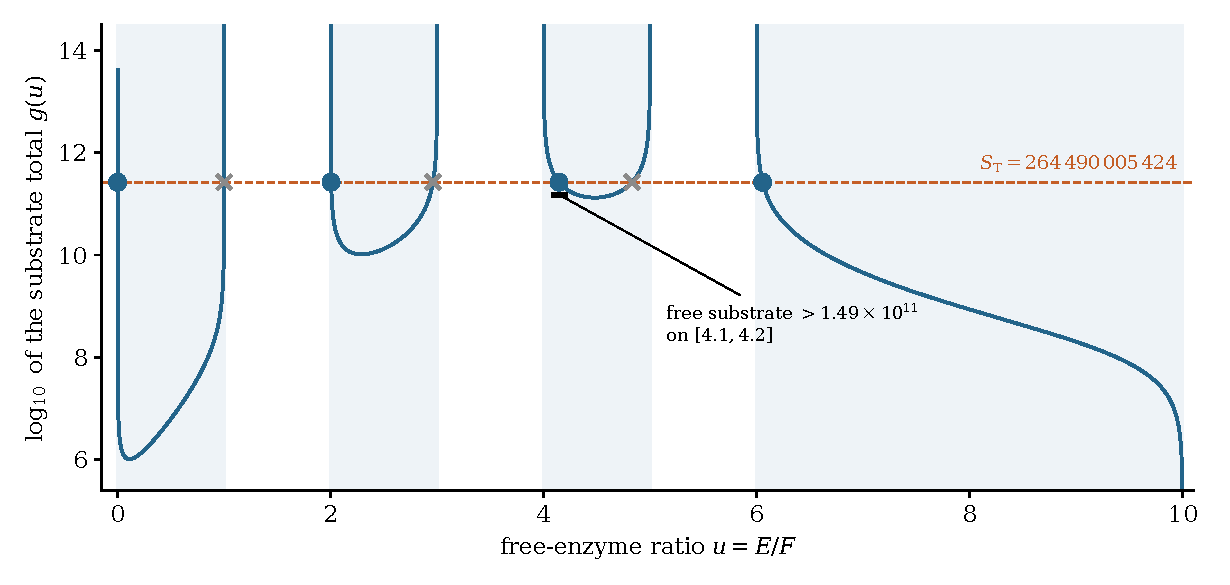
\includegraphics[width=0.86\textwidth]{figures/equilibrium_curve.pdf}
\caption{The final source. The substrate total \(g(u)\) along the curve of equilibria with
\((\ET,\FT)=(10,1)\), on the four admissible intervals (shaded), and the seven equilibria at
\(\ST=264\,490\,005\,424\): sinks (dots) on the decreasing parts and unstable equilibria
(crosses) on the increasing parts. The short black bar is the lower bound of
Proposition~\ref{prop:obstruction} for the free substrate on \(4.1\le u\le4.2\). The curve is
drawn from high-precision floating-point evaluation; the positions and the stability of the
equilibria are certified separately.}
\label{fig:curve}
\end{figure}

\begin{proposition}[Computer-assisted: seven equilibria, four sinks]\label{prop:foursinks}
For the final source:
\begin{enumerate}
\item[\textup{(a)}] The eliminant \eqref{eq:elim} has degree \(15\) and exactly eight positive
roots, all simple. Seven of them are admissible,
\[
 u\approx1.529\times10^{-7},\ 0.99988,\ 2.00464,\ 2.96146,\ 4.14463,\ 4.83103,\ 6.05627 ,
\]
and the eighth, \(u\approx10.000002>r\), is not. Hence the class contains exactly seven
positive equilibria, and all are nondegenerate.
\item[\textup{(b)}] The first, third, fifth and seventh are hyperbolic sinks: for each there is
an explicit rational symmetric matrix \(P_i\) and a rational lower-triangular matrix \(R_i\)
with positive diagonal such that \(R_iP_iR_i^T\) and \(-(J^TP_i+P_iJ)\) are strictly
diagonally dominant with positive diagonal, with margins above \(9/10\), for every Jacobian
\(J\) of the \(31\)-dimensional class chart evaluated on an isolating interval of the root.
\item[\textup{(c)}] The other three equilibria have index \(-1\) and are unstable.
\end{enumerate}
In particular \(C_3\ge4\). The same statements hold for the original source.
\end{proposition}
\begin{proof}
(a) and (b) are verified by the replay program: real-root isolation for the integer eliminant,
the sign conditions of \eqref{eq:reconstruct} at the roots, and interval evaluation of the
state, the Jacobian and the two matrix inequalities. Diagonal dominance of \(R_iP_iR_i^T\)
gives \(P_i>0\) since \(R_i\) is invertible, and Lyapunov's theorem gives that \(J\) is
Hurwitz. For nondegeneracy, note that along the curve of equilibria with \(\ET,\FT\) fixed,
\(\cP(u)=(\ST-g(u))\,uLM\), so a root with \(LM\ne0\) is simple exactly when \(g'(u)\ne0\). In
the coordinates \((u,s,F)\) of Lemma~\ref{lem:regular} the derivative of \((\ET,\FT)\) with
respect to \((s,F)\) has determinant \(uFM\ne0\) by \eqref{eq:threetotals}, so \(\cT|_\cZ\) is
regular at the equilibrium if and only if \(g'(u)\ne0\). (c) By Lemma~\ref{lem:degree} the
seven indices add up to one; four of them are \(+1\), so the remaining three, which are
\(\pm1\), are all \(-1\). Then \(\det(-J)<0\), so \(J\) has a positive real eigenvalue.
\end{proof}
High-precision eigenvalue computations (diagnostics, not used in the proof) agree: the three
unstable equilibria have exactly one unstable direction. Double-precision eigenvalues are
unreliable for this source because of its extreme separation of time scales, which is why the
certificates use exact arithmetic throughout.

\subsection{Readout and operating contract}
As readout take the total amount of fully phosphorylated substrate,
\(R=S_{[3]}+\sum_{\hd e=[3]}Y_e\). At the four sinks
\begin{equation}\label{eq:readouts}
 R/\ST\approx3.31\times10^{-21},\quad 0.316355,\quad 0.558771,\quad 0.670451 ,
\end{equation}
with all gaps larger than \(0.1116\) (Figure~\ref{fig:capacity}). The first value is positive,
not zero. The separation of the four labels is therefore \emph{moderate}: this example is not
crowded in the sense of Section~\ref{sec:crowding}, and its cost must not be attributed to four
states being squeezed into a scalar interval.

\begin{figure}[tbp]
\centering
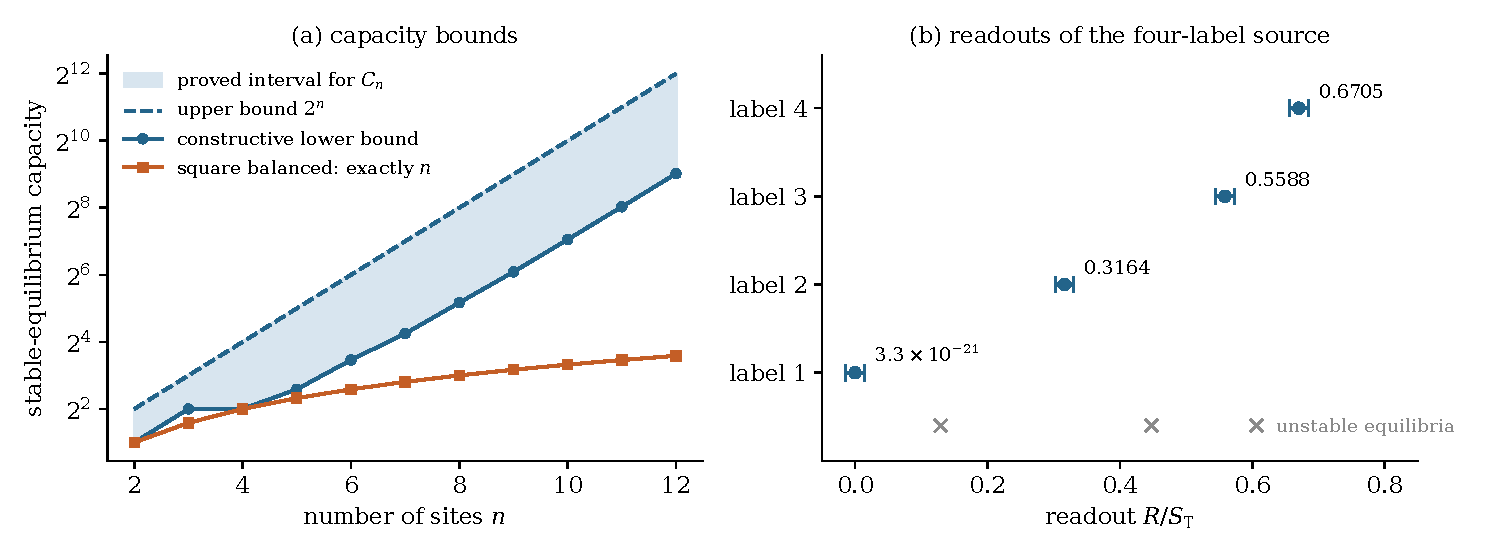
\includegraphics[width=\textwidth]{figures/capacity_readout.pdf}
\caption{(a) Theorem~\ref{thm:capacity}: the proved interval for \(C_n\), the constructive
lower bound (including \(C_3\ge4\)) and the exact capacity \(n\) of square-balanced rates. No
uncomputed value of \(C_n\) is plotted. (b) Readouts \eqref{eq:readouts} of the four sinks of
the final source with the observation tolerance of Proposition~\ref{prop:contract} (one eighth
of the smallest gap), and the readouts of the three unstable equilibria.}
\label{fig:capacity}
\end{figure}

\begin{proposition}[Computer-assisted: operating contract]\label{prop:contract}
For the final source with all rate constants divided by \(50000000/10001\) \textup{(}the model
clock\textup{)}, let \(P_i\) be as in Proposition~\textup{\ref{prop:foursinks}} and define
\(\overline p_i,\underline p_i,\mu,K,\varrho_i\) by the rational formulas of
Appendix~\textup{\ref{app:certificates}}, with \(\varepsilon_{\mathrm{obs}}\) equal to one
eighth of the smallest readout gap and \(C_i\) the local bound \eqref{eq:localC}. Then the
hypotheses of Theorem~\textup{\ref{thm:finite}} and Corollary~\textup{\ref{cor:contract}} hold
with
\[
 \Omega=\lceil\text{right-hand side of \eqref{eq:budget}}\rceil+1\approx1.31\times10^{100}.
\]
Every retention bound is below \(0.00105\) and every recovery bound below \(0.008987\). Four
explicit vectors of \(34\) nonnegative integer counts with the exact totals
\((10\,\Omega,\Omega,\ST\Omega)\) lie in the preparation sets \(\mathsf B_i\).
\end{proposition}
The constant \(C_i\) in Theorem~\ref{thm:finite} may be bounded crudely, using
\(S_I\le\ST\), \(E,C_e\le\ET\), \(F,Y_e\le\FT\), or locally, using that on the ellipsoid
\(D_i\) every species satisfies
\begin{equation}\label{eq:localC}
 x_j\le\overline{x_j^*}+\|\cT_j\|_1\,\varrho_i ,
\end{equation}
where \(\overline{x_j^*}\) is an upper bound of the equilibrium value and \(\cT_j\) the row of
the affine chart map for species \(j\). The local bound changes nothing else in the proof of
Theorem~\ref{thm:finite}, which already works with the stopped process. It lowers the
sufficient \(\Omega\) by a factor \(5.0\times10^{6}\) for the original source and
\(5.4\times10^{9}\) for the final source.

\subsection{Physical units and certified resources}
To compare with laboratory scales, let the concentration unit be
\(C_0=10^{-6}\,\mathrm M/\ST\), so that the total substrate concentration is
\(1\,\mu\mathrm M\), and let the time unit be \(1\,\mathrm s\). An association constant \(a\)
then corresponds to \(a/C_0\) and a unimolecular constant \(b\) to \(b\,\mathrm s^{-1}\). We
slow each source uniformly until its largest association constant is
\(10^{6}\,\mathrm M^{-1}\mathrm s^{-1}\) and its largest unimolecular constant at most
\(100\,\mathrm s^{-1}\); for the final source the factor is \(2.4\times10^{12}\). By
Proposition~\ref{prop:clock} this changes all times and leaves \(\Omega\) unchanged. The
volume is \(\Omega/(N_{\!A}C_0)\) with \(N_{\!A}=6.02214076\times10^{23}\,\mathrm{mol}^{-1}\).
Table~\ref{tab:resources} lists the result.

\begin{table}[tbp]
\centering\small
\caption{Certified \emph{sufficient} resources for the contract of
Corollary~\ref{cor:contract}, with total substrate \(1\,\mu\mathrm M\) and the common upper
limits on rate constants. Entries are base-10 logarithms. Each storage horizon is
\(100\,\trec\) of its own source, so the horizons are not the same absolute duration. None of
the columns describes a feasible assay.}
\label{tab:resources}
\begin{tabular}{lrrr}
\toprule
Quantity & Original, global \(C_i\) & Original, local \(C_i\) & Final, local \(C_i\)\\
\midrule
Substrate molecules & 143.534 & 136.835 & 111.541\\
Kinase molecules & 133.111 & 126.413 & 101.118\\
Phosphatase molecules & 132.111 & 125.413 & 100.118\\
Volume (litres) & 125.754 & 119.055 & 93.761\\
Recovery time \(\trec\) (seconds) & 38.706 & 38.706 & 31.152\\
Storage horizon \(T\) (seconds) & 40.706 & 40.706 & 33.152\\
\bottomrule
\end{tabular}
\end{table}

Relative to the first column, the final source lowers the sufficient number of molecules by a
factor of about \(10^{32}\) and the certified recovery time by \(3.6\times10^{7}\). These are
large improvements of an existence certificate, and they leave it far from any experiment:
\(3.5\times10^{111}\) substrate molecules, \(5.8\times10^{93}\) litres and a recovery time of
\(1.4\times10^{31}\) seconds. For comparison, \(20\,\mu\mathrm L\) at \(1\,\mu\mathrm M\)
contains \(1.2\times10^{13}\) substrate molecules. This is a comparison with a sufficient
bound; it does not show that a small volume cannot hold four labels in another design. Units
cannot remove the problem: at \(1\,\mu\mathrm M\) substrate the phosphatase concentration is
\(1\,\mu\mathrm M/\ST\approx3.8\times10^{-18}\,\mathrm M\), and after the slowing the largest
unimolecular constant is about \(4\times10^{-9}\,\mathrm s^{-1}\).

As an exploratory screen for a cell-free assay one may ask for enzyme-to-substrate ratios
between \(0.01\) and \(1\), association constants between \(10^{3}\) and
\(10^{6}\,\mathrm M^{-1}\mathrm s^{-1}\), unimolecular constants between \(0.01\) and
\(100\,\mathrm s^{-1}\), recovery within \(10^{3}\,\mathrm s\), and a normalized readout error
of \(0.01\); in vitro studies of ERK2 and its phosphatases work at comparable enzyme and
substrate concentrations over minutes \cite{TaylorERK2019}. These are design assumptions, not
measured ranges for the \(72\) constants of this source, and no such study provides a
calibrated four-label error law. Both sources fail the screen by many orders of magnitude in
the ratios, in the lower kinetic limits and in the recovery time.

\begin{figure}[tbp]
\centering
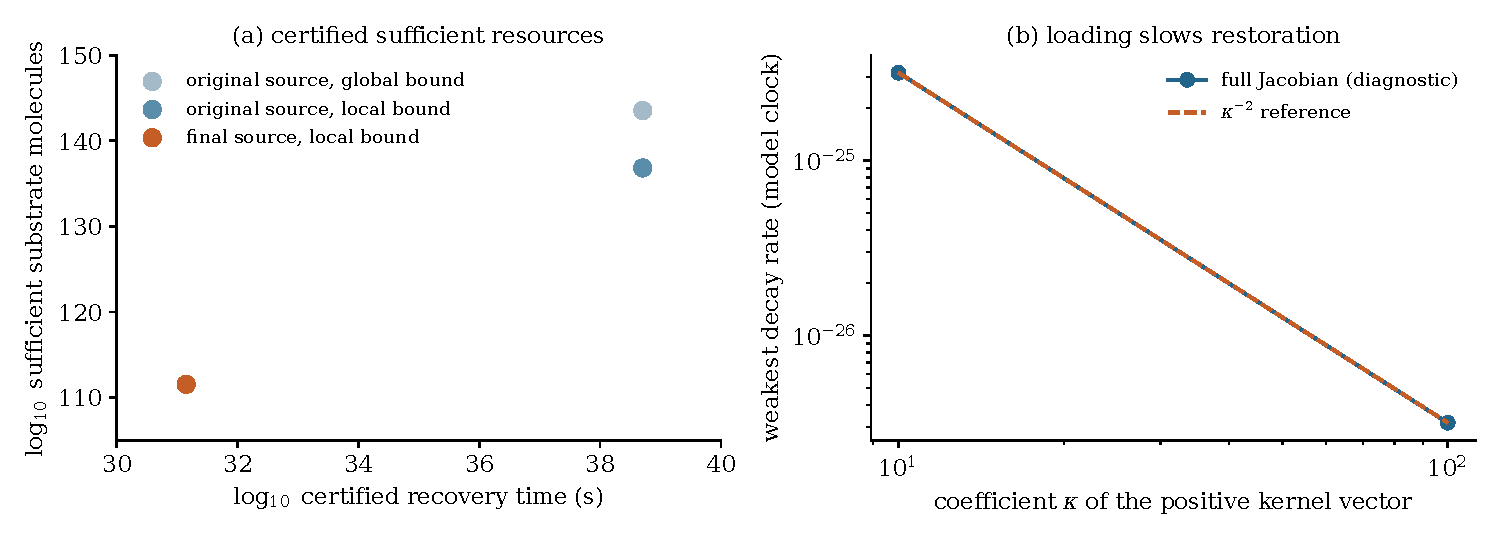
\includegraphics[width=\textwidth]{figures/cost.pdf}
\caption{(a) The three columns of Table~\ref{tab:resources}; the points are certified
sufficient values under the protocol \(T=100\,\trec\), not an optimized trade-off curve. (b)
Floating-point diagnostic for Remark~\ref{rem:loadingcost}(a): with the effective rates and the
target \eqref{eq:target} fixed, increasing the multiple \(\kappa\) of the kernel vector from
\(10\) to \(100\) lowers the weakest decay rate at the third sink by a factor \(99.999\).
Neither panel is a stochastic simulation or a calibrated prediction.}
\label{fig:cost}
\end{figure}

\subsection{Where the cost comes from}
Several losses are distinct, and only some of them are artefacts of the analysis.

\emph{Intrinsic slowness.} High-precision eigenvalues (diagnostics) give weakest decay rates
of \(1.4\times10^{-17}\), \(1.3\times10^{-27}\), \(9.1\times10^{-29}\) and
\(4.4\times10^{-28}\,\mathrm s^{-1}\) at the four sinks of the final source in the slowed
physical clock. This is the \(\eta/\kappa^2\) mechanism of Remark~\ref{rem:loadingcost}, made
worse by the association limit (Figure~\ref{fig:cost}b). No Lyapunov function can certify
faster recovery than the dynamics has.

\emph{Certificate losses.} The certified rates \(\lambda_i\) are smaller than the intrinsic
ones by factors between \(59\) and \(246\). The bounds
\(\overline p_i/\underline p_i\) on the condition numbers of the metrics \(P_i\) lie between
\(10^{19}\) and \(10^{31}\), and the radii \(\varrho_i\) between \(10^{-22}\) and
\(10^{-17}\) in the chart; both enter \eqref{eq:budget} through \(v_i=\underline p_i\varrho_i^2\).
Global propensity bounds cost a further factor between \(5\times10^{6}\) and
\(3\times10^{10}\) in \(C_i\), which
\eqref{eq:localC} removes. Better metrics, or exponential rather than quadratic test
functions, could reduce these losses. They cannot repair the first item or the next.

\emph{Concentration geometry.} In both sources the enzymes are almost completely bound and
nearly all substrate is free, and \(\ET/\ST=3.8\times10^{-11}\). For the family of designs to
which both sources belong this is forced:

\begin{proposition}[Ratio obstruction]\label{prop:obstruction}
Fix the effective rates \eqref{eq:example-rates}, the target \eqref{eq:target} and
\((\ET,\FT)=(10,1)\). For every choice of positive loadings satisfying \eqref{eq:target}, and
every \(\ST\), an equilibrium with \(4.1\le u\le4.2\) has free substrate
\[
 \sum_IS_I=\frac{(10-u)A(u)}{u\prod_{j=1}^6(u-j)}
 \ \ge\ \frac{2260898025826008319}{15168384}>1.49\times10^{11},
 \qquad\text{hence}\qquad \frac{\ET}{\ST}<6.8\times10^{-11}.
\]
\end{proposition}
\begin{proof}
By \eqref{eq:reconstruct}, \(\sum_IS_I=sA\) depends on the loadings only through \(L\), which is
fixed. On \([4.1,4.2]\) we have \(L>0\) and
\(L(u)\le\prod_j\max\{|4.1-j|,|4.2-j|\}\), while \(A(u)\ge A(4.1)\) because \(A\) has
nonnegative coefficients, and \((10-u)/u\ge5.8/4.2\). The resulting rational number is the one
displayed, and \(\ST\ge\sum_IS_I\).
\end{proof}
The third sink of both sources lies in this interval. Thus no choice of loadings, and in
particular no shift along the kernel of Lemma~\ref{lem:kernel}, brings this family into the
range of enzyme-to-substrate ratios of the screen. The proposition is an obstruction for the
stated family only. The effective rates, the position of the roots of the target relative to
the tree weights, the retained branch and the enzyme totals are all outside its hypotheses;
changing the enzyme totals, for instance, alters the shape of \(g(u)\) and hence the set of
coexisting equilibria, and has not been explored. Multiplying all tree weights and the target
by a common factor changes nothing.

\subsection{Robustness and driving thresholds for the example}
\begin{proposition}[Computer-assisted]\label{prop:example-robust}
For the final source, with rational bounds \(b_G,d_G\) computed on the ellipsoids \(D_i\):
\textup{(a)} every rate list whose \(72\) constants differ from the given ones by relative
errors at most \(10^{-99}\) has four hyperbolic sinks, one in each \(D_i'\), with pairwise
disjoint decoder intervals; \textup{(b)} the reversible extension \eqref{eq:reversible} has
four such sinks for every \(0<\vartheta\le10^{-102}\), that is, for a hydrolysis potential of
\(204\ln10\approx469.7\) in units of \(\kB T\).
\end{proposition}
\begin{proof}
Proposition~\ref{prop:robust} with the certified minima \(4.2\times10^{-99}\) and
\(4.0\times10^{-102}\) of the right-hand side of \eqref{eq:robust} over the four sinks.
\end{proof}
These margins measure the conditioning of the example and the conservatism of
Proposition~\ref{prop:robust}. They are not experimentally meaningful tolerances, the threshold
is not a minimum free-energy requirement (cellular ATP hydrolysis provides roughly
\(20\,\kB T\) \cite{Qian2007}), and the finite-molecule contract has not been recomputed for
the perturbed or the reversible source.

\section{Discussion}\label{sec:discussion}

\paragraph{Which kinetic structure permits many states.}
The capacity of the distributive cube is governed by the cycle structure of its
\emph{effective} rates. If every elementary square is balanced, the equilibria are those of a
single chain and at most \(n\) of them are stable, regardless of the \(2^n\) phosphoforms and
of the loadings. If squares are unbalanced, the loadings become an exponentially large space of
design parameters for the scalar equation on the equilibrium curve, and
\(\Theta(2^n)\) stable states are possible. The proofs keep these two ingredients apart: the
number of crossings is programmed linearly through the loadings, while transverse stability
comes from the saturated family and does not depend on the programming. Rank alone, a scalar
root count alone, or a Hamiltonian path through the cube would not establish stable capacity
for the full mass-action network.

\paragraph{Structure is not operation.}
Theorem~\ref{thm:finite} shows that any finite set of hyperbolic sinks becomes a set of
reliable labels at some finite system size, so stable-equilibrium capacity is an upper bound on
what can be stored in equilibrium labels and is attainable in principle. The price is not
controlled by the capacity theorems. In crowded families it is controlled by
Theorem~\ref{thm:action} and Corollary~\ref{cor:tradeoff}; in the loading construction, by the
\(\eta/\kappa^2\) slowing and the positivity burden of Remark~\ref{rem:loadingcost}; and in the
worked example, additionally by very conservative certificates. We have tried to keep three
kinds of statement apart: theorems with explicit scope, exact computations for one source, and
floating-point diagnostics. In particular the figures \(10^{111}\) molecules and
\(10^{31}\) seconds are sufficient for our certificate and are not claimed to be necessary,
even for this source.

\paragraph{What the example teaches for design.}
The obstruction of Proposition~\ref{prop:obstruction} and the diagnostics of
Section~\ref{sec:example} suggest that the next design step is not a finer readout, a larger
volume or a sharper probability bound, but a different equilibrium geometry: effective rates
and a target whose retained branches have moderate free-substrate levels at moderate enzyme
totals, found by continuation of the common-total branches while monitoring the smallest
readout gap, the weakest eigenvalue and the size of the loadings. A low-parameter family with
four robust sinks would be more informative than another isolated point among \(72\) rate
constants. Whether a three-site substrate with shared enzymes can hold four robust, readable
and quickly recovering states at physical rates and inventories is open, and nothing in this
paper suggests that it is impossible.

\paragraph{Open problems.}
(1) Determine \(C_n\); already \(4\le C_3\le8\) is open, as is the maximal number of positive
equilibria, between \(7\) and \(15\) for \(n=3\). (2) Find an intermediate structural condition,
weaker than square balance, that bounds the capacity polynomially in \(n\). (3) Prove an exit
law for crowded states that is uniform along joint sequences \((\delta,\Omega)\), or a global
basin-exit law. (4) Replace the quadratic certificates by test functions adapted to the slow
direction; preliminary computations with exponential test functions improve the retention
part of the budget by about nine orders of magnitude but not the recovery part. (5) Recompute
the finite-molecule contract for the reversible extension at a declared hydrolysis potential,
with ATP turnover accounted for. (6) Analyse a writing protocol. (7) Extend the capacity
results to mechanisms with shared complexes, processive steps or several enzymes.

\paragraph{Data and code availability.}
The source bundle of this paper contains the exact rational data of the example, the
certificate replay program, the figure scripts and the three Lean files; see
Appendix~\ref{app:certificates}.
